%%%%%%%%%%%%%%%%%%%%%%%%%%%%%%%%%%%%%%%%%%%%%%%%%%%%%%%%%%%
%                                                         %
%       This is documentation for the IFJ project.        %
%                                                         %
%%%%%%%%%%%%%%%%%%%%%%%%%%%%%%%%%%%%%%%%%%%%%%%%%%%%%%%%%%%


%------------------------------------------------%
%	    CONFIGURATION + IMPORTED PACKAGES        %
%------------------------------------------------%
\documentclass[10pt,a4paper,titlepage]{article}
\usepackage[english]{babel}
\usepackage[utf8]{inputenc}
\usepackage[margin=100pt]{geometry}


\usepackage{graphicx}   % Import pictures
\usepackage{ragged2e}   % fullfill paragraphs

\begin{document}
%-----------------------------------------%
%	            TITLE PAGE                %
%-----------------------------------------%
\begin{titlepage}

\begin{center}
% Headings
\textsc{\LARGE Brno University of technology}\\[0.5cm]
\textsc{\large Faculty of Information Technology}\\[7cm]

% Title - lines
{ \huge \bfseries IFJ project}\\[0.3cm]
{ \Large \bfseries documentation}\\[0.4cm]
{\bfseries xbenes49, xbolsh00, xpolan09}\\[10cm]

% Date
\today
\end{center}

\end{titlepage}
\newpage

%-----------------------------------------%
%	            CHAPTERS                  %
%-----------------------------------------%

\setcounter{page}{1}
\pagenumbering{arabic}

\section{Lexical analysis}

\begin{justify}
We did the scanner in two ways: singlethread and multithread work. Both variants work on the basis of a state machine.
The state machine was created on a basis of regular expression designs for each type of phrasems:
integer, real number (decimal point, positive or negative exponent), string, operator, identifier, keyword, comment.

The multithread scanner implementation used separate thread, read bytes from input, generates tokens and pushes
them to the queue. The parser then reads from the queue and processess the tokens in it. At some moment of multithread
implementing, we have come to the decision, that the singlethread scanner would be better, since we have got one member off.

For the purpose of decomposition, the structure of the lexical analyzer was divided into several subprograms
that implemented individual parts.
\end{justify}

%%%%% getNumber %%%%%
\begin{justify}
Numbers, decimal and exponential numbers are scanned in the function \textit{getNumber()}.
\end{justify}
\begin{center}
  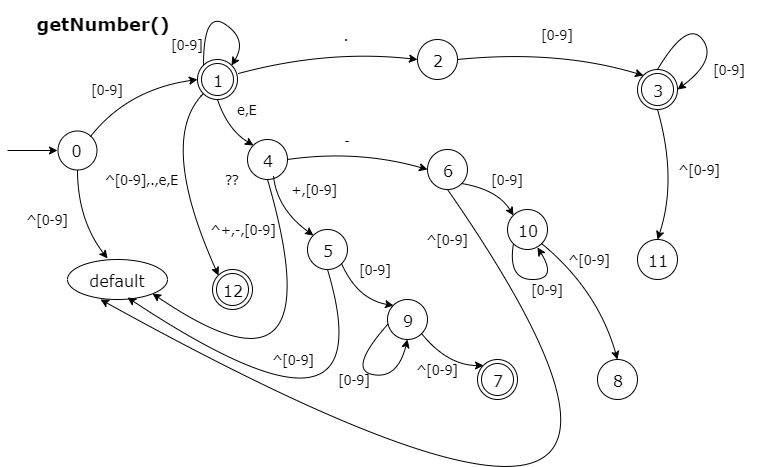
\includegraphics[width=0.7\textwidth]{img/getNumber.png}
\end{center}

%%%%% getString %%%%%
\begin{justify}
Strings are scanned in the function \textit{getString()}.
\end{justify}
\begin{center}
  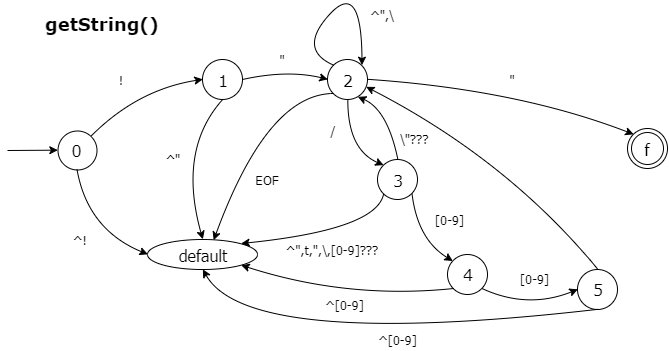
\includegraphics[width=0.7\textwidth]{img/getString.png}
\end{center}

%%%%% getComment %%%%%
\begin{justify}
The comments are scanned in the function \textit{getComment()}. We have simplified the "//" with "\textasciitilde".
\end{justify}
\begin{center}
  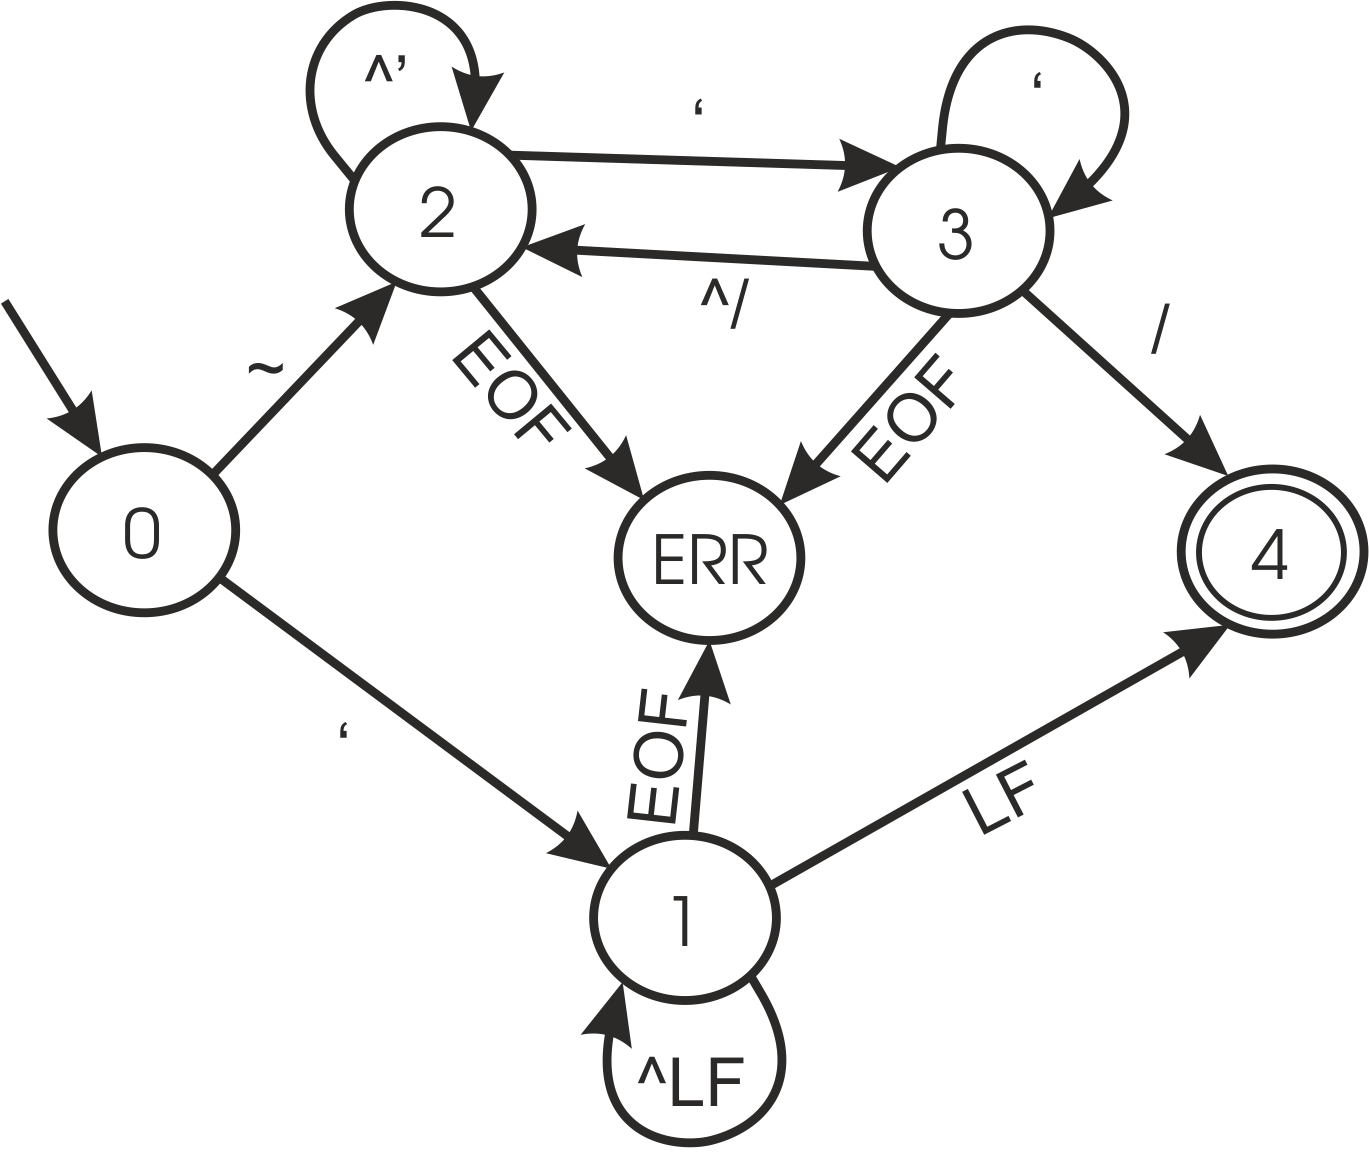
\includegraphics[width=0.7\textwidth]{img/getComment.png}
\end{center}

%%%%% getIdentifier %%%%%
\begin{justify}
Identifiers and keywords are scanned in the function \textit{getIdentifier()}.
\end{justify}
\begin{center}
  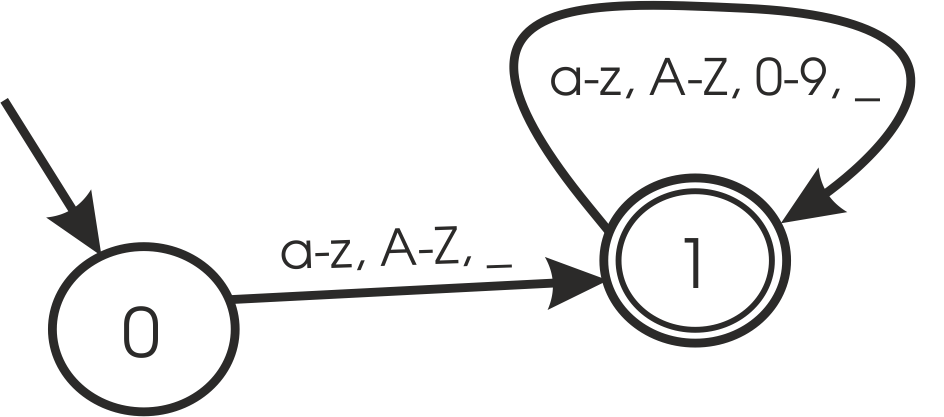
\includegraphics[width=0.7\textwidth]{img/getIdentifier.png}
\end{center}

%%%%% getOperator %%%%%
\begin{justify}
Operators are scanned in the function \textit{getOperator()}
\end{justify}
\begin{center}
  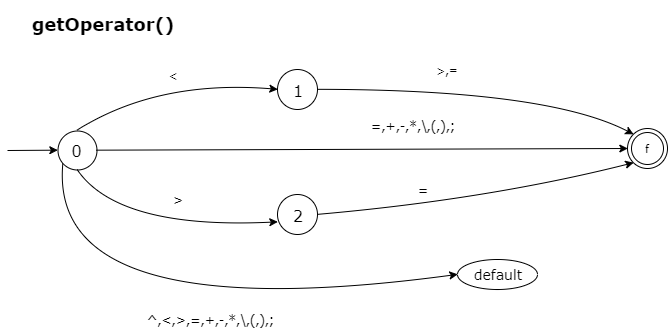
\includegraphics[width=0.7\textwidth]{img/getOperator.png}
\end{center}

\begin{justify}
To simplify the implementation, we use a wrapper modul \textit{io.h} to
be able to return bytes back to the input with the function \textit{returnByte()}.
\end{justify}

\newpage
% ------------------------------------------------------- %

\section{Parser}

% LL table
{\scriptsize
%{\footnotesize
  \begin{center}
    \begin{tabular}{ | l | c  c  l | } \hline
      1  & $<$GlobalBlock$>$              & $\rightarrow$ & $<$FunctionDeclaration$>$ $<$GlobalBlock$>$ \\ \hline
      2  & $<$GlobalBlock$>$              & $\rightarrow$ & $<$FunctionDefinition$>$ $<$GlobalBlock$>$ \\ \hline
      3  & $<$GlobalBlock$>$              & $\rightarrow$ & $<$Scope$>$ $<$GlobalBlock$>$ \\ \hline
      4  & $<$GlobalBlock$>$              & $\rightarrow$ & $\varepsilon$ \\ \hline
      5  & $<$FunctionDeclaration$>$      & $\rightarrow$ & {\it declare} $<$FunctionHeader$>$ \\ \hline
      6  & $<$FunctionDefinition$>$       & $\rightarrow$ & $<$FunctionHeader$>$ $<$Block$>$ $<$EndFunction$>$ \\ \hline
      7  & $<$FunctionHeader$>$           & $\rightarrow$ & {\it function} $<$FSymbol$>$ {\it (} $<$Parameters$>$ {\it )} {\it as} $<$DataType$>$ {\it \$} \\ \hline
      8  & $<$Scope$>$                    & $\rightarrow$ & {\it scope} {\it \$} $<$Block$>$ $<$EndScope$>$ \\ \hline
      9  & $<$FSymbol$>$                  & $\rightarrow$ & {\it id} \\ \hline
      10 & $<$VSymbol$>$                  & $\rightarrow$ & {\it id} \\ \hline
      11 & $<$DataType$>$                 & $\rightarrow$ & {\it string} \\ \hline
      12 & $<$DataType$>$                 & $\rightarrow$ & {\it double} \\ \hline
      13 & $<$DataType$>$                 & $\rightarrow$ & {\it integer} \\ \hline
      14 & $<$EndFunction$>$              & $\rightarrow$ & {\it end} {\it function} {\it \$} \\ \hline
      15 & $<$EndScope$>$                 & $\rightarrow$ & {\it end} {\it scope} {\it \$} \\ \hline
      16 & $<$Parameters$>$               & $\rightarrow$ & $<$VSymbol$>$ {\it as} $<$DataType$>$ $<$MoreParameters$>$ \\ \hline
      17 & $<$Parameters$>$               & $\rightarrow$ & $\varepsilon$ \\ \hline
      18 & $<$MoreParameters$>$           & $\rightarrow$ & {\it ,} $<$Parameters$>$ \\ \hline
      19 & $<$MoreParameters$>$           & $\rightarrow$ & $\varepsilon$ \\ \hline
      20 & $<$Block$>$                    & $\rightarrow$ & $<$VariableDefinition$>$ $<$Block$>$ \\ \hline
      21 & $<$Block$>$                    & $\rightarrow$ & $<$Assignment$>$ $<$Block$>$ \\ \hline
      22 & $<$Block$>$                    & $\rightarrow$ & $<$Input$>$ $<$Block$>$ \\ \hline
      23 & $<$Block$>$                    & $\rightarrow$ & $<$Print$>$ $<$Block$>$ \\ \hline
      24 & $<$Block$>$                    & $\rightarrow$ & $<$Condition$>$ $<$Block$>$ \\ \hline
      25 & $<$Block$>$                    & $\rightarrow$ & $<$Cycle$>$ $<$Block$>$ \\ \hline
      26 & $<$Block$>$                    & $\rightarrow$ & $<$Return$>$ $<$Block$>$ \\ \hline
      27 & $<$VariableDefinition$>$       & $\rightarrow$ & {\it dim} $<$VSymbol$>$ {\it as} $<$DataType$>$ $<$VariableInitialization$>$ {\it \$} \\ \hline
      28 & $<$VariableInitialization$>$   & $\rightarrow$ & {\it =} $<$Expression$>$ {\it \$} \\ \hline
      29 & $<$VariableInitialization$>$   & $\rightarrow$ & $\varepsilon$ \\ \hline
      30 & $<$Assignment$>$               & $\rightarrow$ & $<$VSymbol$>$ {\it =} $<$AssignmentValue$>$ {\it \$} \\ \hline
      31 & $<$AssignmentValue$>$          & $\rightarrow$ & $<$Expression$>$ \\ \hline
      32 & $<$AssignmentValue$>$          & $\rightarrow$ & $<$FunctionCall$>$ \\ \hline
      33 & $<$FunctionCall$>$             & $\rightarrow$ & $<$FSymbol$>$ {\it (} $<$Arguments$>$ {\it )} {\it \$} \\ \hline
      34 & $<$Arguments$>$                & $\rightarrow$ & $<$Expression$>$ $<$MoreArguments$>$ \\ \hline
      35 & $<$Arguments$>$                & $\rightarrow$ & $\varepsilon$ \\ \hline
      36 & $<$MoreArguments$>$            & $\rightarrow$ & {\it ,} $<$Arguments$>$ \\ \hline
      37 & $<$MoreArguments$>$            & $\rightarrow$ & $\varepsilon$ \\ \hline
      38 & $<$Input$>$                    & $\rightarrow$ & {\it input} $<$VSymbol$>$ {\it \$} \\ \hline
      39 & $<$Print$>$                    & $\rightarrow$ & {\it print} $<$Expression$>$ {\it ;} $<$PrintParameters$>$ {\it \$} \\ \hline
      40 & $<$PrintParameters$>$          & $\rightarrow$ & $<$Expression$>$ {\it ;} $<$PrintParameters$>$ \\ \hline
      41 & $<$PrintParameters$>$          & $\rightarrow$ & $\varepsilon$ \\ \hline
      42 & $<$Condition$>$                & $\rightarrow$ & {\it if} $<$Logic$>$ {\it then} {\it \$} $<$Block$>$ {\it else} {\it \$} $<$Block$>$ $<$EndIf$>$ \\ \hline
      43 & $<$Logic$>$                    & $\rightarrow$ & $<$Expression$>$ $<$ComparisonOperator$>$ $<$Expression$>$ \\ \hline
      44 & $<$ComparisonOperator$>$       & $\rightarrow$ & {\it $<$} \\ \hline
      45 & $<$ComparisonOperator$>$       & $\rightarrow$ & {\it $<=$} \\ \hline
      46 & $<$ComparisonOperator$>$       & $\rightarrow$ & {\it $>$} \\ \hline
      47 & $<$ComparisonOperator$>$       & $\rightarrow$ & {\it $>=$} \\ \hline
      48 & $<$ComparisonOperator$>$       & $\rightarrow$ & {\it $=$} \\ \hline
      49 & $<$ComparisonOperator$>$       & $\rightarrow$ & {\it $<>$} \\ \hline
      50 & $<$EndIf$>$                    & $\rightarrow$ & {\it end} {\it if} {\it \$} \\ \hline
      51 & $<$Cycle$>$                    & $\rightarrow$ & {\it do} {\it while} $<$Logic$>$ {\it \$} $<$Block$>$ $<$EndCycle$>$ \\ \hline
      52 & $<$EndCycle$>$                 & $\rightarrow$ & {\it loop} {\it \$} \\ \hline
      53 & $<$Return$>$                   & $\rightarrow$ & {\it return} $<$Expression$>$ {\it \$} \\ \hline
      54 & $<$Expression$>$               & $\rightarrow$ & {\bf calling precedent analysis...} \\ \hline
    \end{tabular}
  \end{center}
}

\end{document}
